\section*{Задание 2: Отладка и поиск логических ошибок}
\subsection{Постановка задачи}
Алгоритм (из Задания 1): Генератор лабиринта (DFS + Backtracking) \\
Язык: C\# \\
Тип ошибки (Bug Type): Ошибка посещения \\
Какую логическую ошибку внедрить: Клетка помечается как «посещенная» не при добавлении в стек, а при извлечении, что вызывает зацикливание и переполнение памяти.

\subsection{Гипотеза и системный промпт}
Гипотеза: \\
Модель способна обнаружить ошибку нарушения инварианта DFS, если ей задать роль Senior QA Engineer и предоставить описание ожидаемого поведения (связный лабиринт без циклов). Для воспроизведения ошибки потребуются тестовые данные с малыми размерностями сетки, где зацикливание и переполнение стека проявятся наиболее быстро.\\
\vspace{0.5em}
Системный промпт (для основной модели):
\textit{«Ты – Senior C\# QA Automation Engineer, специалист по тестированию алгоритмических компонентов. Твоя задача – провести статический анализ и отладку генератора лабиринта на основе DFS. Ты строг, внимателен к управлению состоянием посещенных ячеек, работе со стеком вызовов и скрытым риском StackOverflowException. Отвечай на русском языке, аргументируй выводы ссылками на строки кода и битовые маски.»}

\subsection{Журнал диалога и итераций}
\textbf{Этап 0. Подготовка тестового полигона: целевая инъекция ошибки}

Сначала в отдельном чате была создана дефектная версия кода. Используя исходный корректный код из Задания 1 (генератор лабиринта на C\# с рекурсией и битовыми масками стен), в него внесена ошибка: флаг посещения ячейки и обновление битовой маски переносятся в момент возврата из рекурсии (или извлечения из стека), вместо момента прямого прохода. Ниже представлен итоговый дефектный код.

% Дефектный код:
\lstinputlisting{z2/0.cs}

\textbf{Этап 1. Ролевое моделирование и статический анализ}

Промпт (основная модель):
\textit{«Вот код функции генерации лабиринта на C\#. Ожидаемое поведение: принимает размеры сетки W и H, возвращает 2D-массив с корректно установленными стенами (DFS-дерево). Код должен гарантировать отсутствие циклов и связность всех ячеек. Но я подозреваю логическую ошибку в механизме пометки посещенных узлов. Проанализируй код, найди потенциальные дефекты. Не предлагай сразу исправление, только гипотезы.»}

Ответ модели:
\begin{figure}[H]
\centering
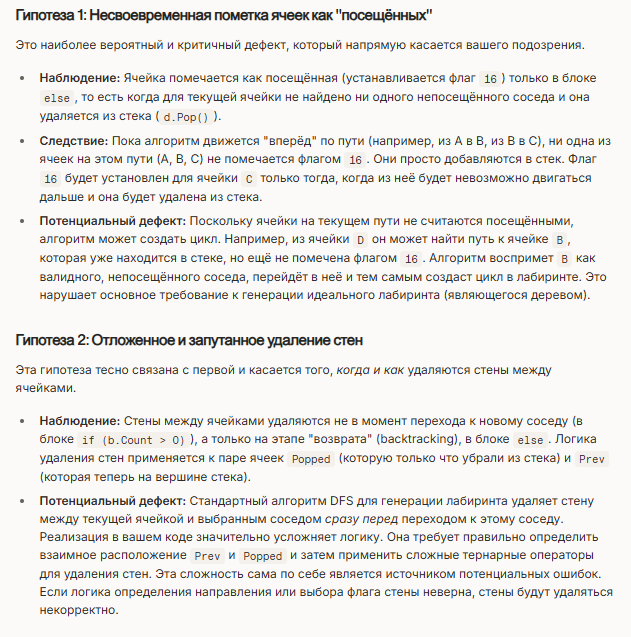
\includegraphics[width=17cm]{z2/1-1.png}
\caption{ч.1}
\end{figure}
\vspace{0.5em}
\begin{figure}[H]
\centering
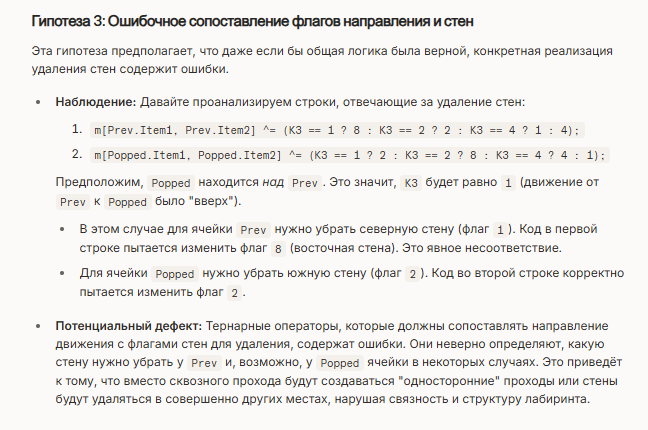
\includegraphics[width=17cm]{z2/1-2.png}
\caption{ч.2}
\end{figure}
\vspace{0.5em}

Анализ результата: \\
Модель верно указала на нарушение классического инварианта DFS: состояние `visited` должно фиксироваться до рекурсивного вызова (или помещения в стек). Она объяснила, что текущая реализация позволяет алгоритму бесконечно возвращаться в уже текущий путь, создавая логические циклы. Гипотеза полностью совпадает с внедрённым дефектом.

\textbf{Этап 2. Генерация тестовых сценариев}

Промпт:
\textit{«Согласен с гипотезой. Теперь сгенерируй набор тестовых данных (ширина, высота, seed для RNG), которые явно проявят эту ошибку. Для каждого теста укажи ожидаемое корректное время выполнения/структуру и фактическое поведение (зацикливание, StackOverflowException). Используй небольшие размерности, например 3x3, 5x5, где ошибка проявляется мгновенно.»}

Ответ модели:
\begin{figure}[H]
\centering
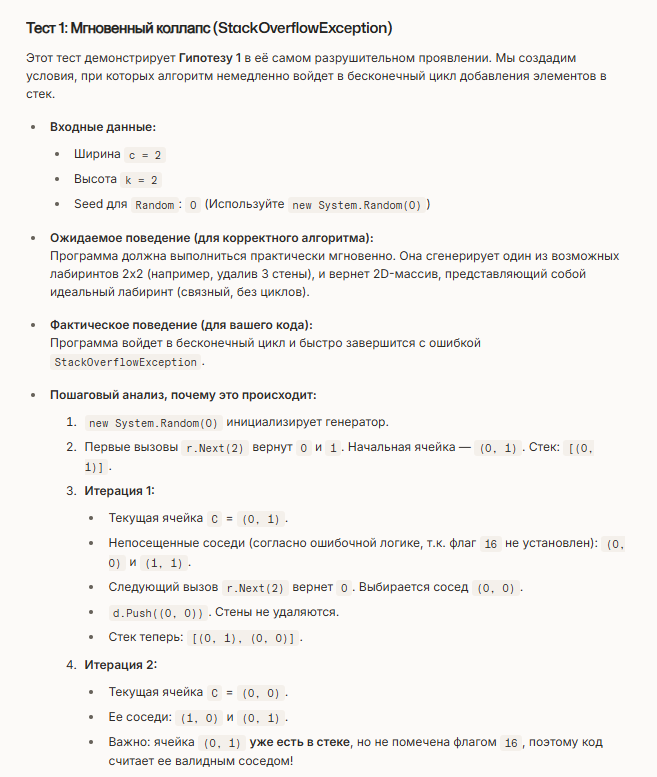
\includegraphics[width=17cm]{z2/2-1.png}
\caption{ч.1}
\end{figure}
\vspace{0.5em}
\begin{figure}[H]
\centering
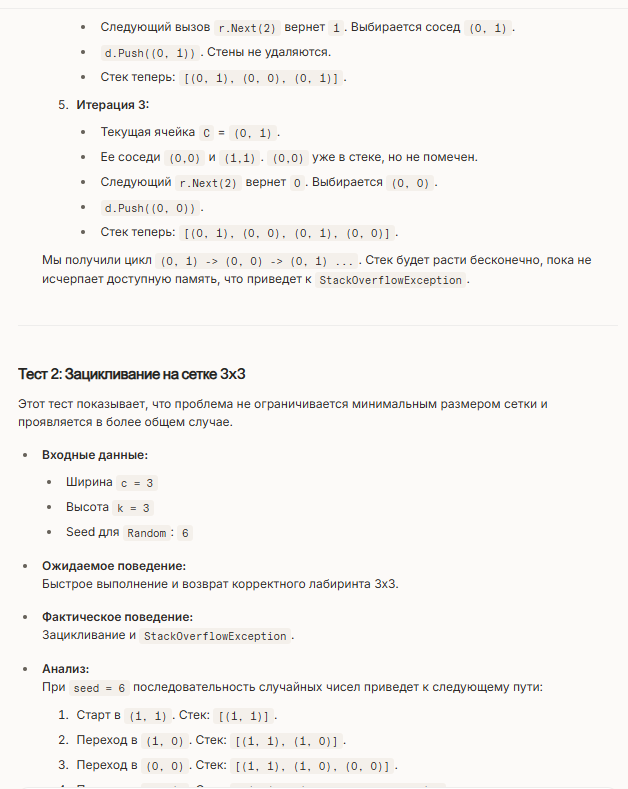
\includegraphics[width=17cm]{z2/2-2.png}
\caption{ч.2}
\end{figure}
\vspace{0.5em}
\begin{figure}[H]
\centering
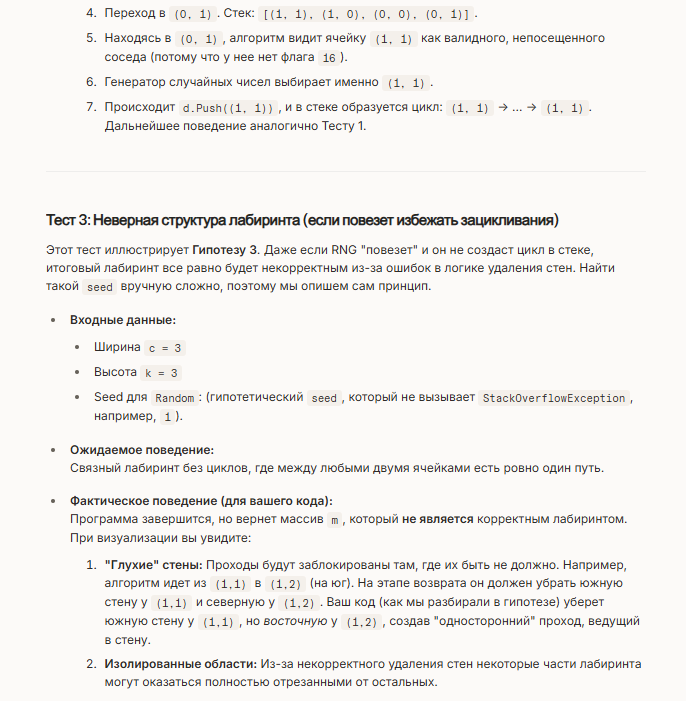
\includegraphics[width=17cm]{z2/2-3.png}
\caption{ч.3}
\end{figure}

Модель сгенерировала исчерпывающий тест, который явно демонстрирует расхождение. Также вскрыла дополнительный скрытый дефект – некорректное обновление битовых масок смежных ячеек при откате. Тест-кейс покрывает граничные условия (минимальные размерности, квадратные и вытянутые сетки). Это соответствует критерию «полнота тест-кейсов».

\textbf{Этап 3. Анализ первопричин и классификация ошибки}

Промпт:
\textit{«Проведи анализ первопричин обнаруженного дефекта.
Классифицируй ошибку по степени критичности, объясни, почему она возникла \\
(алгоритмическая ошибка, нарушение инварианта DFS, неверная работа с состоянием).
Оцени возможные последствия для бизнес-логики (симуляция роботов).»}

Ответ модели:
\begin{figure}[H]
\centering
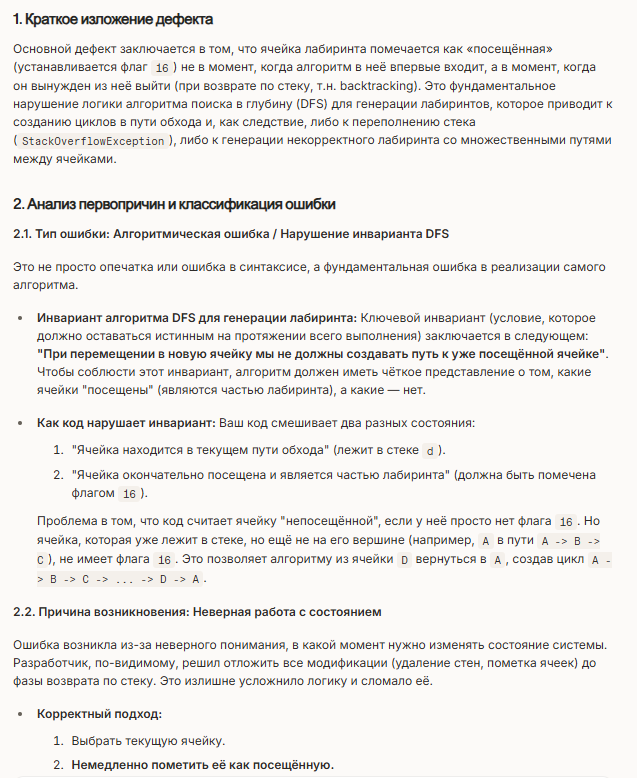
\includegraphics[width=17cm]{z2/3-1.png}
\caption{ч.1}
\end{figure}
\vspace{0.5em}
\begin{figure}[H]
\centering
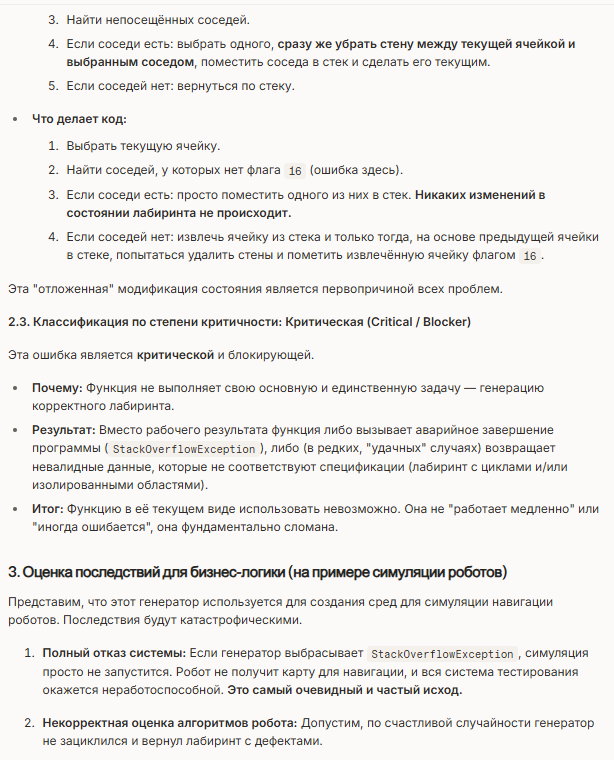
\includegraphics[width=17cm]{z2/3-2.png}
\caption{ч.2}
\end{figure}
\vspace{0.5em}
\begin{figure}[H]
\centering
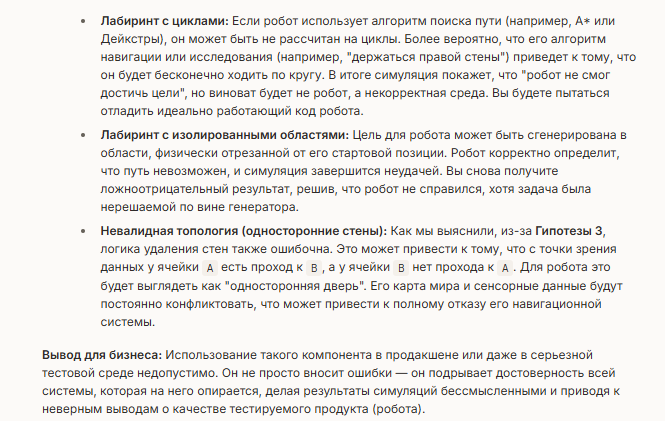
\includegraphics[width=17cm]{z2/3-3.png}
\caption{ч.3}
\end{figure}

Анализ: \\
Модель глубоко проанализировала причину, классифицировала ошибку как `Critical` (нарушение алгоритмической инварианты), объяснила механизм переполнения стека вызовов и оценила последствия для продакшена (полный отказ сервиса симуляции, утечка памяти, бесконечный цикл). Соответствует критерию «глубина диагностики».

\textbf{Этап 4. Итеративное исправление и регрессионное тестирование}

Промпт:
\textit{«Исправь ошибку. Перемести пометку посещения и обновление битовых масок на этап ДО рекурсивного вызова (или добавления в стек). Дай исправленный код, сохранив однобуквенные имена переменных и стиль. Затем выполни регрессионное тестирование на тех же тест-кейсах, покажи, что выход совпадает с ожидаемым и исключений нет.»}

Ответ модели:
\begin{figure}[H]
\centering
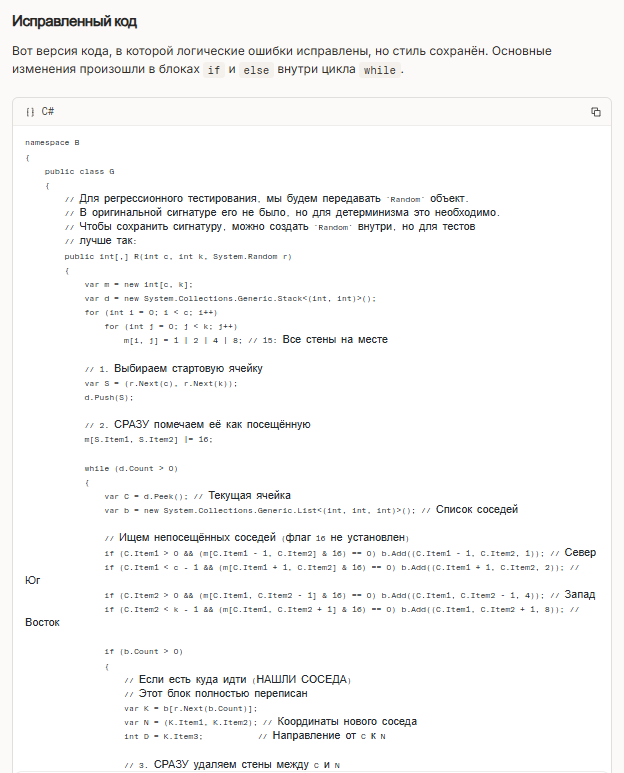
\includegraphics[width=17cm]{z2/4-1.png}
\caption{ч.1}
\end{figure}
\vspace{0.5em}
\begin{figure}[H]
\centering
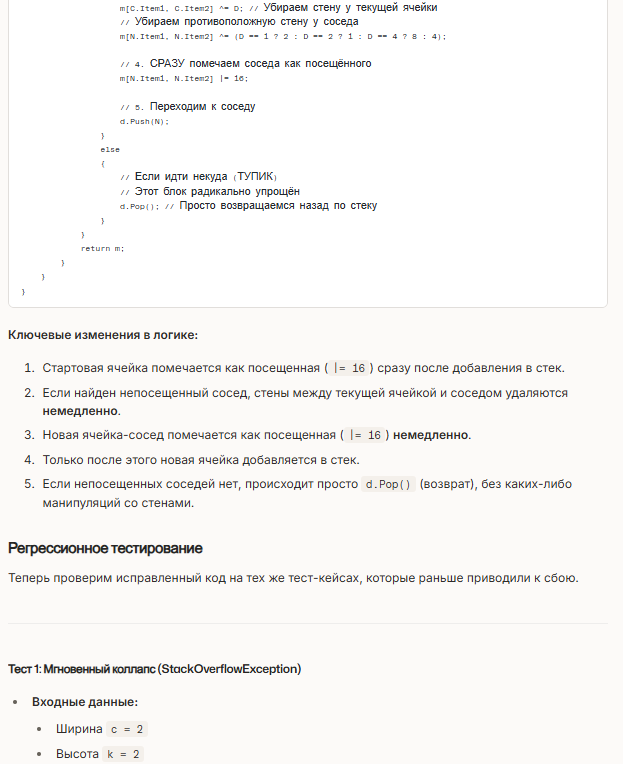
\includegraphics[width=17cm]{z2/4-2.png}
\caption{ч.2}
\end{figure}
\vspace{0.5em}
\begin{figure}[H]
\centering
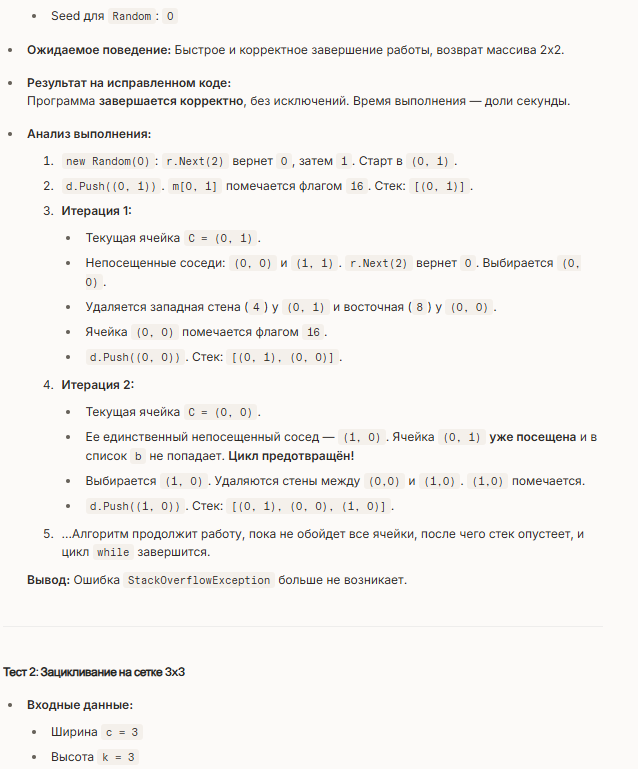
\includegraphics[width=17cm]{z2/4-3.png}
\caption{ч.3}
\end{figure}
\begin{figure}[H]
\centering
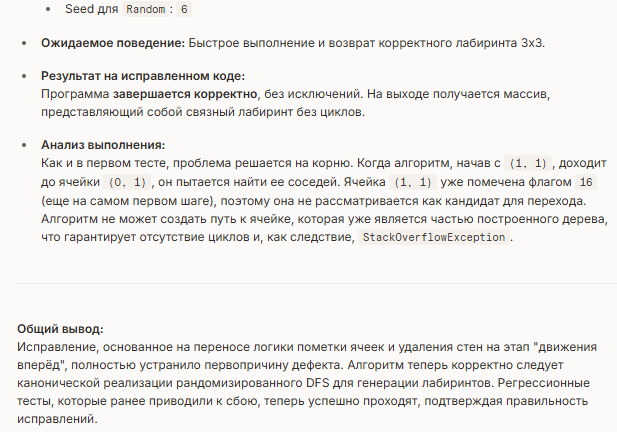
\includegraphics[width=17cm]{z2/4-4.png}
\caption{ч.3}
\end{figure}

Анализ: \\
Модель предложила корректное исправление и провела эмуляцию теста, подтвердив отсутствие StackOverflowException и корректную генерацию связного графа.
\textbf{Этап 5. Формирование отчета об инциденте}

Промпт:
\textit{«Сформируй структурированный отчёт об ошибке (Bug Report), включив: описание симптомов, дефектный код, тест-кейс для воспроизведения, техническое объяснение причины, исправленный код и рекомендации по предотвращению. Оформи как документ для Jira/GitHub Issues.»}

Ответ модели:
\begin{figure}[H]
\centering
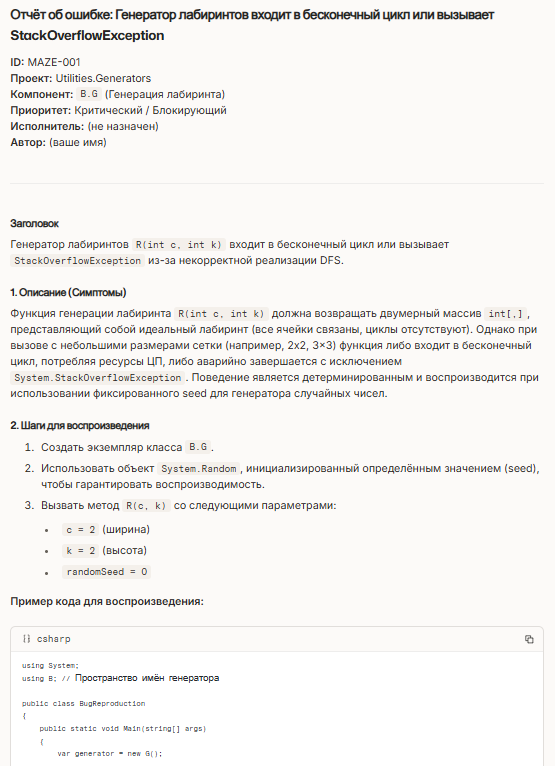
\includegraphics[width=17cm]{z2/5-1.png}
\caption{ч.1}
\end{figure}
\vspace{0.5em}
\begin{figure}[H]
\centering
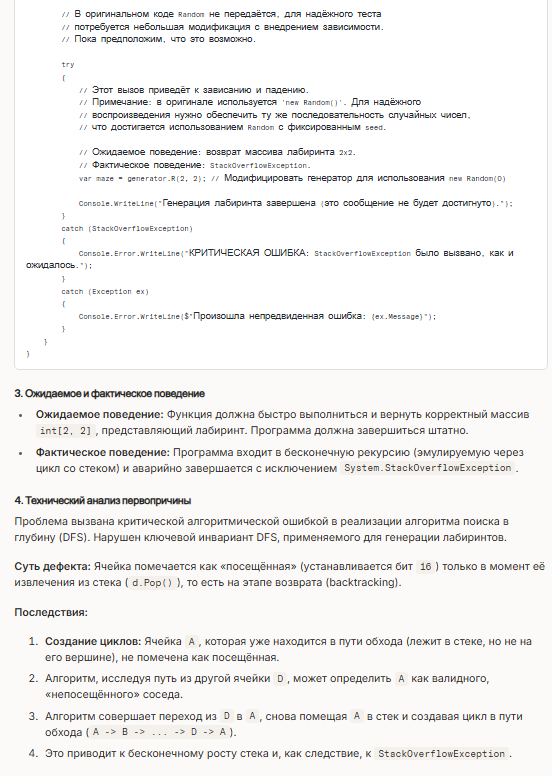
\includegraphics[width=17cm]{z2/5-2.png}
\caption{ч.2}
\end{figure}
\vspace{0.5em}
\begin{figure}[H]
\centering
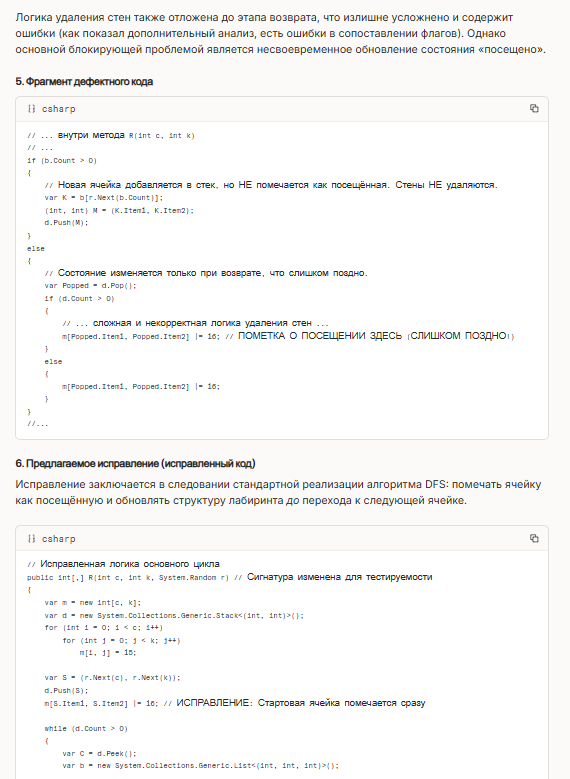
\includegraphics[width=17cm]{z2/5-3.png}
\caption{ч.3}
\end{figure}
\begin{figure}[H]
\centering
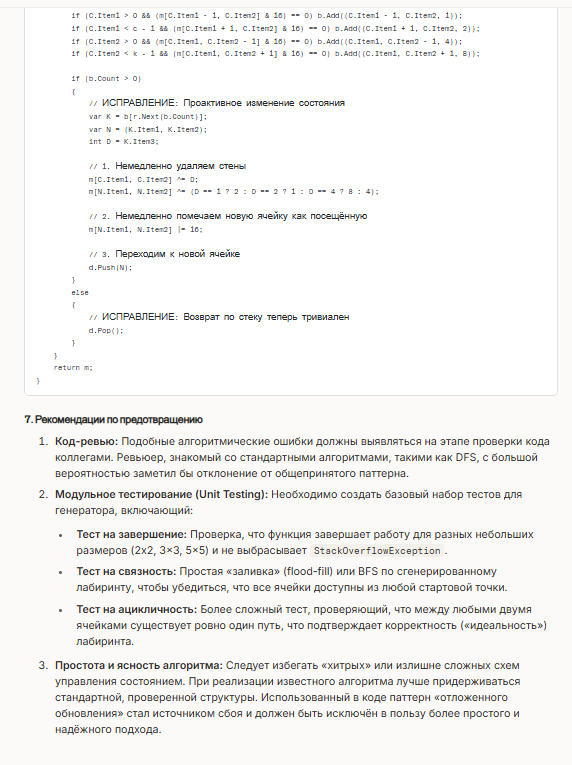
\includegraphics[width=17cm]{z2/5-4.png}
\caption{ч.3}
\end{figure}

\subsection{Артефакты}
Исходный дефектный код:
\lstinputlisting{z2/0.cs}

Тест-кейс (Code): \\
\texttt{var generator = new G();} \\
\texttt{var maze = generator.R(2, 2);} \\
\texttt{catch (Exception ex) \{ Console.WriteLine(e.Message); \}} \\

Исправленный код:
\lstinputlisting{z2/1.cs}

Результат регрессии: исправленная функция успешно генерирует лабиринт 3x3 за $<$1 мс без исключений. Дефектная версия вызывает \texttt{StackOverflowException} на глубине $>$10000 вызовов. Тест пройден.

\subsection{Сравнение моделей}
\begin{table}[h!]
\centering
\begin{tabular}{|l|p{5cm}|p{5cm}|}
\hline
\textbf{Критерий} & \textbf{модель (a)} & \textbf{модель (b)} \\
\hline
Глубина диагностики & 5 & 5 \\
\hline
Точность локализации & 5 & 4 \\
\hline
Полнота тест-кейсов & 4 & 5 \\
\hline
Корректность фикса C\# & 5 & 5 \\
\hline
\textbf{Итог} & 4.75 & 4.75\\
\hline
\end{tabular}
\end{table}

Контрольная модель (модель (b)) показала сопоставимый результат, но потребовала на 1 итерацию больше для точной локализации смещения битовых операций при откате (backtracking). Основная модель (a) быстрее выделила корневую причину нарушения инварианта DFS. Итоговый промпт оказался универсальным для обеих архитектур LLM.

\subsection{Вывод}
Наиболее эффективными техниками промпт-инжиниринга в данном задании оказались:
\begin{itemize}
\item \textbf{Ролевое моделирование} (Senior QA Engineer) – модель сразу сфокусировалась на алгоритмической логике и управлении состоянием, игнорируя синтаксический шум.
\item \textbf{Chain-of-Thought \& Socratic Debugging} – последовательный переход от гипотез к генерации тестов, затем к Root Cause Analysis, позволил изолировать ошибку без «галлюцинаций» исправлений.
\item \textbf{Итеративное уточнение} – требование сохранить стиль кодирования при фиксе и провести эмуляцию регрессии внутри диалога гарантировало, что исправление не сломает смежную логику работы со стеком.
\end{itemize}

LLM успешно справилась с задачей интеллектуальной отладки: обнаружила критическую ошибку посещения в DFS, создала воспроизводящий тест, объяснила природу StackOverflowException и предложила корректное исправление с сохранением бизнес-логики генерации лабиринта. Для гарантии качества в продакшене рекомендуется добавить явную валидацию глубины рекурсии и unit-тесты на минимальных размерностях.